% Created:  Wed 09 Jul 2014 03:00 PM
% Modified: Wed 09 Jul 2014 03:00 PM
% @author Josh Wainwright
% File name : clusters.tex

\section{Cluster Analysis}
\label{sec:cluster_analysis}

Cluster analysis is the grouping of a set of objects or items in a spatially or
informationally logical way such that the items that are placed in the same
group are more similar to each other than they are to the objects in the other
groups in the set. These groups shall be called \emph{clusters}. When dealing
with images, the clustering that is of interest is based on spatial location,
i.e., clusters should be composed of objects that are close together in the
image and clusters should be separated by regions of emptiness or background
level noise.

One of the primary reasons for chosing the quadtree method over the simple grid
methods was that the simple act of placing the objects, in this case
coordinates of data points, into the quadtree starts the process of analysing
the data. Since the points end up in a tree structure with the number of points
closely separated being on the lowest levels of the tree, the data is already
clustered in a way.

There are a number of alternative methods of identifying clusters in images.

% Created:  Mon 30 Jun 2014 05:32 PM
% @author Josh Wainwright
% File name : rolling-ball.tex

\section{Rolling Ball Analysis}
\label{sec:rolling_ball_analysis}

The accessible surface area (ASA) algorithm, also known as the ``Rolling Ball
Method'', is a technique used in image processing for describing the outer
limit of a cluster of points. It is derived from biological molecules analysis
where it describes the surface area of a molecule that is accessible to a
solvent.

The rolling ball method can be used to analyse a cluster of points by imagining
a solid ball that sits against one of the outer-most points. From here it is
``rolled'' around the cluster such that it is always touching at least one
point. Once the ball has reached the point it started at, the line that the ball
traced is reduced in size by the radius of the ball. This line then represents
the outer limit of the cluster.

The size of the ball must be chosen depending on the average separation of the
points within the cluster.

\begin{figure}[tbhp]
	\centering
	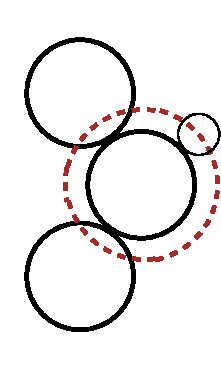
\includegraphics[width=4.2cm]{rolling-ball.pdf}

	\caption[Rolling ball method for cluster detection.]{The rolling ball
		method for cluster detection provides a way of identifying clusters, as
		inspired by molecular biology. A very simple implementation can be fast
		but is not particularly successful at finding clusters unless the data
		points are very dense and there is no noise.}\label{fig:rolling-ball}
\end{figure}

A simple approximation of this technique can be acheived by using the same
\texttt{open}-ing and \texttt{close}-ing processes as are described in
Section~\ref{sec:simple_grid_method}.

